% ============================================================
% 讲义 — 人教版高中数学必修第一册 第4章
% 编译命令：xelatex -interaction=nonstopmode 高一必修1_第4章_指数函数与对数函数.tex
% ============================================================
\documentclass[12pt, a4paper]{ctexart}
\usepackage[margin=2.2cm]{geometry}
\usepackage{amsmath, amssymb}
\usepackage{enumitem}
\usepackage{tcolorbox}
\usepackage{booktabs}
\usepackage{array}
\usepackage{fancyhdr}
\usepackage{xcolor}
\usepackage{tikz}
\usepackage{hyperref}
\usepackage{graphicx}
\usepackage{multirow}
\usepackage{pgfplots}
\pgfplotsset{compat=1.18}

% 颜色定义
\definecolor{mainblue}{RGB}{41, 98, 168}
\definecolor{lightblue}{RGB}{230, 240, 255}
\definecolor{tipgreen}{RGB}{34, 139, 87}
\definecolor{lightgreen}{RGB}{235, 250, 240}
\definecolor{warnred}{RGB}{200, 50, 50}
\definecolor{lightred}{RGB}{255, 240, 240}
\definecolor{examorange}{RGB}{210, 120, 20}
\definecolor{lightorange}{RGB}{255, 248, 235}
\definecolor{apppurple}{RGB}{120, 60, 170}
\definecolor{lightpurple}{RGB}{245, 238, 255}

% 页眉页脚
\pagestyle{fancy}
\fancyhf{}
\fancyhead[L]{\small\textcolor{mainblue}{\textbf{人教版高中必修第一册 · 第4章}}}
\fancyhead[R]{\small\textcolor{mainblue}{指数函数与对数函数}}
\fancyfoot[C]{\small —\ \thepage\ —}
\renewcommand{\headrulewidth}{0.6pt}
\renewcommand{\headrule}{\hbox to\headwidth{\color{mainblue}\leaders\hrule height \headrulewidth\hfill}}
\renewcommand{\footrulewidth}{0pt}

% tcolorbox 样式
\newtcolorbox{knowledgebox}[1][]{%
  colback=lightblue, colframe=mainblue,
  fonttitle=\bfseries\large, title=#1,
  arc=3mm, boxrule=0.8pt,
  left=8pt, right=8pt, top=6pt, bottom=6pt
}

\newtcolorbox{tipbox}[1][]{%
  colback=lightgreen, colframe=tipgreen,
  fonttitle=\bfseries, title=#1,
  arc=2mm, boxrule=0.6pt,
  left=6pt, right=6pt, top=4pt, bottom=4pt
}

\newtcolorbox{warnbox}[1][]{%
  colback=lightred, colframe=warnred,
  fonttitle=\bfseries, title=#1,
  arc=2mm, boxrule=0.6pt,
  left=6pt, right=6pt, top=4pt, bottom=4pt
}

\newtcolorbox{examplebox}[1][]{%
  colback=lightorange, colframe=examorange,
  fonttitle=\bfseries, title=#1,
  arc=3mm, boxrule=0.8pt,
  left=8pt, right=8pt, top=6pt, bottom=6pt
}

\newtcolorbox{appbox}[1][]{%
  colback=lightpurple, colframe=apppurple,
  fonttitle=\bfseries, title=#1,
  arc=3mm, boxrule=0.8pt,
  left=8pt, right=8pt, top=6pt, bottom=6pt
}

\setCJKmainfont{Hiragino Sans GB}
\setCJKsansfont{Heiti SC}

\begin{document}

% ============ 标题页 ============
\begin{center}
{\Huge\bfseries\textcolor{mainblue}{第4章\quad 指数函数与对数函数}}\\[12pt]
{\Large\textcolor{gray}{讲\quad 义}}\\[8pt]
\rule{0.6\textwidth}{1pt}\\[8pt]
{\normalsize 适用：人教版\quad 高中必修第一册\quad |\quad 课时：8课时}
\end{center}
\vspace{10pt}


% =============================================================
%  第一部分：知识点讲解
% =============================================================
\section*{\textcolor{mainblue}{一、知识点讲解}}

% ==================== 4.1 ====================
\subsection*{4.1\quad $n$次根式与分数指数幂}

\begin{knowledgebox}[$n$次方根]
如果 $x^n = a$（$n \in \mathbb{N}^*$，$n \geq 2$），那么 $x$ 叫做 $a$ 的 \textbf{$n$次方根}。

\begin{itemize}[leftmargin=2em]
  \item 当 $n$ 为\textbf{奇数}时，正数的 $n$ 次方根是一个正数，负数的 $n$ 次方根是一个负数，记作 $\sqrt[n]{a}$。
  \item 当 $n$ 为\textbf{偶数}时，正数的 $n$ 次方根有两个，它们互为相反数，分别记作 $\pm\sqrt[n]{a}$。
  \item 负数没有偶次方根。
  \item $0$ 的 $n$ 次方根是 $0$，即 $\sqrt[n]{0}=0$。
\end{itemize}

式子 $\sqrt[n]{a}$ 叫做\textbf{根式}，其中 $n$ 叫做\textbf{根指数}，$a$ 叫做\textbf{被开方数}。
\end{knowledgebox}

\begin{knowledgebox}[$n$次根式的性质]
对于任意正整数 $n$（$n\geq 2$）：
\begin{enumerate}[leftmargin=2em]
  \item $(\sqrt[n]{a})^n = a$ \quad（$a$ 有意义时成立）
  \item 当 $n$ 为奇数时，$\sqrt[n]{a^n} = a$
  \item 当 $n$ 为偶数时，$\sqrt[n]{a^n} = |a|$
\end{enumerate}
\end{knowledgebox}

\begin{knowledgebox}[分数指数幂]
为了统一根式与幂的运算，规定：

\[
\boxed{a^{\frac{m}{n}} = \sqrt[n]{a^m}} \quad (a>0,\ m\in\mathbb{Z},\ n\in\mathbb{N}^*,\ n\geq 2)
\]

即 $a$ 的 $\dfrac{m}{n}$ 次幂，等于 $a$ 的 $m$ 次幂的 $n$ 次方根。

\vspace{4pt}
特别地：$a^{-\frac{m}{n}} = \dfrac{1}{a^{\frac{m}{n}}} = \dfrac{1}{\sqrt[n]{a^m}}\quad (a>0)$
\end{knowledgebox}

\begin{warnbox}[易错提醒]
\begin{itemize}[leftmargin=2em]
  \item $(-2)^{\frac{1}{2}}$ \textbf{无意义}！分数指数幂的底数必须为正数（或零，指数为正时）。
  \item $\sqrt[4]{(-3)^4} = |-3| = 3$，注意偶次根式的结果为非负数。
  \item $a^{\frac{2}{4}} = a^{\frac{1}{2}}$ 是正确的化简，但前提是 $a>0$。
\end{itemize}
\end{warnbox}

% ==================== 4.2 ====================
\subsection*{4.2\quad 指数幂的运算性质}

\begin{knowledgebox}[指数幂运算三大法则]
设 $a>0$，$b>0$，$r,s\in\mathbb{Q}$，则：
\begin{enumerate}[leftmargin=2em]
  \item $\boxed{a^r \cdot a^s = a^{r+s}}$ \quad \textcolor{gray}{（同底数幂相乘，底数不变，指数相加）}
  \item $\boxed{(a^r)^s = a^{rs}}$ \quad \textcolor{gray}{（幂的乘方，底数不变，指数相乘）}
  \item $\boxed{(ab)^r = a^r \cdot b^r}$ \quad \textcolor{gray}{（积的乘方，分别乘方）}
\end{enumerate}
\end{knowledgebox}

\begin{tipbox}[运算小技巧]
\begin{itemize}[leftmargin=2em]
  \item $a^r \div a^s = a^{r-s}$（同底数幂相除，指数相减）
  \item 化简时优先将根式化为分数指数幂：$\sqrt[3]{x^2} = x^{\frac{2}{3}}$
  \item 注意底数相同才能用法则1，底数不同时先化为同底数
\end{itemize}
\end{tipbox}

% ==================== 4.3 ====================
\subsection*{4.3\quad 指数函数的图象与性质}

\begin{knowledgebox}[指数函数的定义]
一般地，函数 \boxed{y = a^x \quad (a>0 \text{ 且 } a \neq 1)} 叫做\textbf{指数函数}，其中 $x$ 是自变量，定义域为 $\mathbb{R}$（全体实数）。
\end{knowledgebox}

\begin{knowledgebox}[指数函数的图象与性质]
\begin{center}
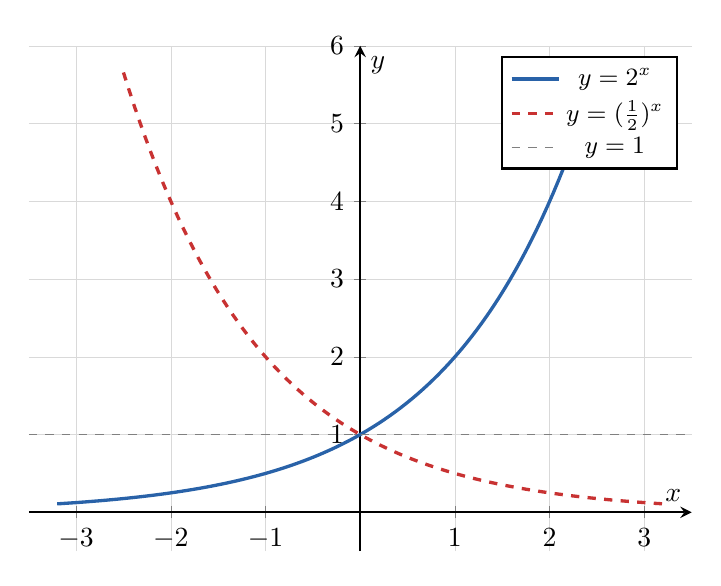
\begin{tikzpicture}
\begin{axis}[
    width=10cm, height=8cm,
    axis lines=middle,
    xlabel={$x$}, ylabel={$y$},
    xmin=-3.5, xmax=3.5,
    ymin=-0.5, ymax=6,
    samples=100,
    grid=both,
    grid style={line width=0.2pt, draw=gray!30},
    legend style={at={(0.98,0.98)}, anchor=north east, font=\small},
    thick,
]
% y = 2^x
\addplot[mainblue, very thick, domain=-3.2:2.5] {2^x};
\addlegendentry{$y=2^x$}
% y = (1/2)^x
\addplot[warnred, very thick, dashed, domain=-2.5:3.2] {0.5^x};
\addlegendentry{$y=(\frac{1}{2})^x$}
% y=1 参考线
\addplot[gray, thin, dashed, domain=-3.5:3.5] {1};
\addlegendentry{$y=1$}
\end{axis}
\end{tikzpicture}
\end{center}

\renewcommand{\arraystretch}{1.3}
\begin{center}
\begin{tabular}{|c|c|c|}
\hline
 & $a>1$ & $0<a<1$ \\
\hline
\textbf{图象} & 从左到右\textbf{上升} & 从左到右\textbf{下降} \\
\hline
\textbf{定义域} & \multicolumn{2}{c|}{$\mathbb{R}$（全体实数）} \\
\hline
\textbf{值域} & \multicolumn{2}{c|}{$(0, +\infty)$} \\
\hline
\textbf{过定点} & \multicolumn{2}{c|}{$(0, 1)$，即 $a^0=1$} \\
\hline
\textbf{单调性} & 在 $\mathbb{R}$ 上\textbf{递增} & 在 $\mathbb{R}$ 上\textbf{递减} \\
\hline
$x>0$ 时 & $y>1$ & $0<y<1$ \\
\hline
$x<0$ 时 & $0<y<1$ & $y>1$ \\
\hline
\end{tabular}
\end{center}
\end{knowledgebox}

\begin{warnbox}[易错提醒]
\begin{itemize}[leftmargin=2em]
  \item $y=2\cdot 3^x$ \textbf{不是}指数函数！指数函数的形式必须是 $y=a^x$，前面系数为 $1$。
  \item $y=3^{2x}$ 可化为 $y=9^x$，是指数函数（底数 $9>1$）。
  \item 指数函数的图象始终在 $x$ 轴\textbf{上方}，即 $y>0$ 恒成立。
  \item 指数函数\textbf{不经过原点}（$x=0$ 时 $y=1\neq 0$）。
\end{itemize}
\end{warnbox}

% ==================== 4.4 ====================
\subsection*{4.4\quad 对数的概念}

\begin{knowledgebox}[对数的定义]
如果 $a^b = N$（$a>0$，$a\neq 1$），那么数 $b$ 叫做以 $a$ 为底 $N$ 的\textbf{对数}，记作：

\[
\boxed{\log_a N = b}
\]

其中 $a$ 叫做\textbf{底数}，$N$ 叫做\textbf{真数}（$N>0$）。

\vspace{4pt}
\textbf{指数式与对数式的互化：}

\[
a^b = N \quad \Longleftrightarrow \quad \log_a N = b
\]
\end{knowledgebox}

\begin{knowledgebox}[两种常用对数]
\begin{itemize}[leftmargin=2em]
  \item \textbf{常用对数}：以 $10$ 为底的对数，记作 $\lg N$，即 $\lg N = \log_{10} N$。
  \item \textbf{自然对数}：以无理数 $\mathrm{e}\approx 2.71828\cdots$ 为底的对数，记作 $\ln N$，即 $\ln N = \log_{\mathrm{e}} N$。
\end{itemize}
\end{knowledgebox}

\begin{knowledgebox}[对数的基本性质]
\begin{enumerate}[leftmargin=2em]
  \item $\log_a 1 = 0$ \quad \textcolor{gray}{（因为 $a^0=1$）}
  \item $\log_a a = 1$ \quad \textcolor{gray}{（因为 $a^1=a$）}
  \item $a^{\log_a N} = N$ \quad \textcolor{gray}{（对数恒等式）}
  \item $\log_a a^n = n$
  \item \textbf{负数和零没有对数}，即真数 $N>0$
\end{enumerate}
\end{knowledgebox}

% ==================== 4.5 ====================
\subsection*{4.5\quad 对数的运算性质}

\begin{knowledgebox}[对数运算法则]
设 $a>0$，$a\neq 1$，$M>0$，$N>0$，则：

\begin{enumerate}[leftmargin=2em]
  \item $\boxed{\log_a(MN) = \log_a M + \log_a N}$ \quad \textcolor{gray}{（积的对数 $=$ 对数之和）}
  \item $\boxed{\log_a \dfrac{M}{N} = \log_a M - \log_a N}$ \quad \textcolor{gray}{（商的对数 $=$ 对数之差）}
  \item $\boxed{\log_a M^n = n\log_a M}$ \quad \textcolor{gray}{（幂的对数 $=$ 指数 $\times$ 对数）}
\end{enumerate}
\end{knowledgebox}

\begin{warnbox}[易错提醒]
\begin{itemize}[leftmargin=2em]
  \item $\log_a(M+N) \neq \log_a M + \log_a N$！和的对数没有简单展开公式。
  \item $\log_a M \cdot \log_a N \neq \log_a(MN)$！注意区分法则。
  \item $\dfrac{\log_a M}{\log_a N} \neq \log_a \dfrac{M}{N}$！除法与商的对数不同。
\end{itemize}
\end{warnbox}

\begin{knowledgebox}[换底公式]
\[
\boxed{\log_a N = \dfrac{\log_b N}{\log_b a}} \quad (a>0,\ a\neq 1,\ b>0,\ b\neq 1,\ N>0)
\]

\textbf{推论}：
\begin{enumerate}[leftmargin=2em]
  \item $\log_a b \cdot \log_b a = 1$
  \item $\log_a b \cdot \log_b c = \log_a c$
  \item $\log_{a^n} b = \dfrac{1}{n}\log_a b$
\end{enumerate}
\end{knowledgebox}

% ==================== 4.6 ====================
\subsection*{4.6\quad 对数函数的图象与性质}

\begin{knowledgebox}[对数函数的定义]
一般地，函数 \boxed{y = \log_a x \quad (a>0 \text{ 且 } a \neq 1)} 叫做\textbf{对数函数}，其中 $x$ 是自变量，定义域为 $(0, +\infty)$，值域为 $\mathbb{R}$。
\end{knowledgebox}

\begin{knowledgebox}[对数函数的图象与性质]
\begin{center}
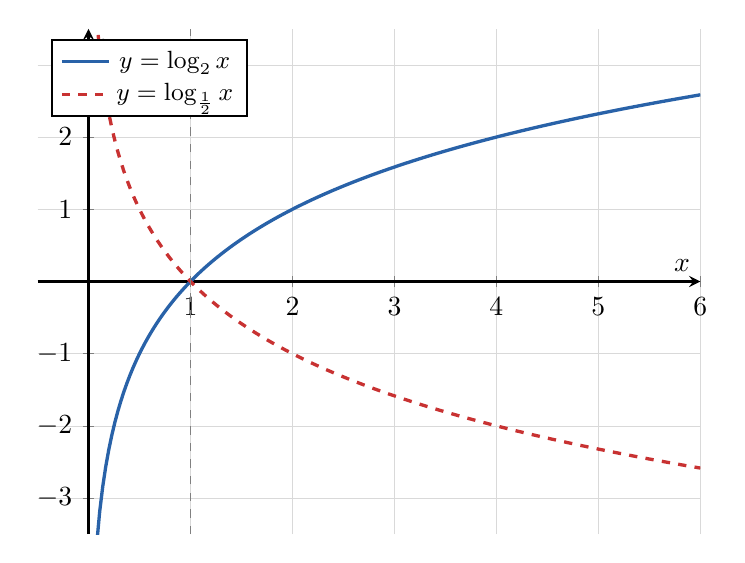
\begin{tikzpicture}
\begin{axis}[
    width=10cm, height=8cm,
    axis lines=middle,
    xlabel={$x$}, ylabel={$y$},
    xmin=-0.5, xmax=6,
    ymin=-3.5, ymax=3.5,
    samples=200,
    grid=both,
    grid style={line width=0.2pt, draw=gray!30},
    legend style={at={(0.02,0.98)}, anchor=north west, font=\small},
    thick,
]
% y = log_2(x)
\addplot[mainblue, very thick, domain=0.08:6] {ln(x)/ln(2)};
\addlegendentry{$y=\log_2 x$}
% y = log_{1/2}(x)
\addplot[warnred, very thick, dashed, domain=0.08:6] {ln(x)/ln(0.5)};
\addlegendentry{$y=\log_{\frac{1}{2}} x$}
% x=1 参考线
\addplot[gray, thin, dashed, domain=-3.5:3.5] coordinates {(1,-3.5) (1,3.5)};
\end{axis}
\end{tikzpicture}
\end{center}

\renewcommand{\arraystretch}{1.3}
\begin{center}
\begin{tabular}{|c|c|c|}
\hline
 & $a>1$ & $0<a<1$ \\
\hline
\textbf{图象} & 从左到右\textbf{上升} & 从左到右\textbf{下降} \\
\hline
\textbf{定义域} & \multicolumn{2}{c|}{$(0, +\infty)$} \\
\hline
\textbf{值域} & \multicolumn{2}{c|}{$\mathbb{R}$} \\
\hline
\textbf{过定点} & \multicolumn{2}{c|}{$(1, 0)$，即 $\log_a 1 = 0$} \\
\hline
\textbf{单调性} & 在 $(0,+\infty)$ 上\textbf{递增} & 在 $(0,+\infty)$ 上\textbf{递减} \\
\hline
$x>1$ 时 & $y>0$ & $y<0$ \\
\hline
$0<x<1$ 时 & $y<0$ & $y>0$ \\
\hline
\end{tabular}
\end{center}
\end{knowledgebox}

% ==================== 4.7 ====================
\subsection*{4.7\quad 指数函数与对数函数互为反函数}

\begin{knowledgebox}[反函数]
指数函数 $y=a^x$ 和对数函数 $y=\log_a x$ \textbf{互为反函数}。

\begin{itemize}[leftmargin=2em]
  \item 它们的图象关于直线 $y=x$ 对称。
  \item $y=a^x$ 的定义域为 $\mathbb{R}$，值域为 $(0,+\infty)$；$y=\log_a x$ 的定义域为 $(0,+\infty)$，值域为 $\mathbb{R}$。定义域和值域恰好互换。
  \item 同底数的指数函数与对数函数单调性相同。
\end{itemize}

\begin{center}
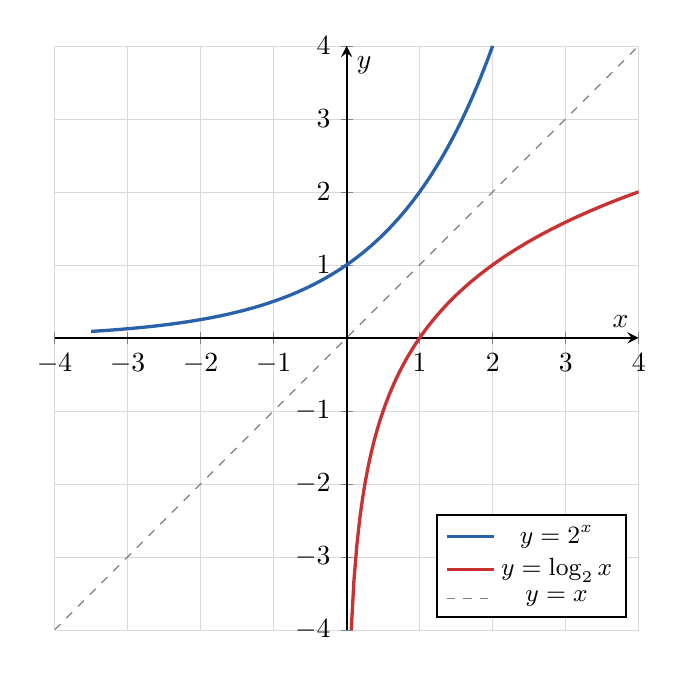
\begin{tikzpicture}
\begin{axis}[
    width=9cm, height=9cm,
    axis lines=middle,
    xlabel={$x$}, ylabel={$y$},
    xmin=-4, xmax=4,
    ymin=-4, ymax=4,
    samples=100,
    grid=both,
    grid style={line width=0.2pt, draw=gray!30},
    legend style={at={(0.98,0.02)}, anchor=south east, font=\small},
    thick,
    axis equal,
]
% y = 2^x
\addplot[mainblue, very thick, domain=-3.5:2] {2^x};
\addlegendentry{$y=2^x$}
% y = log_2(x)
\addplot[warnred, very thick, domain=0.06:4] {ln(x)/ln(2)};
\addlegendentry{$y=\log_2 x$}
% y = x 参考线
\addplot[gray, thin, dashed, domain=-4:4] {x};
\addlegendentry{$y=x$}
\end{axis}
\end{tikzpicture}
\end{center}
\end{knowledgebox}

% ==================== 4.8 ====================
\subsection*{4.8\quad 幂函数简介}

\begin{knowledgebox}[幂函数]
一般地，形如 \boxed{y = x^\alpha}（$\alpha$ 为常数）的函数叫做\textbf{幂函数}，其中 $x$ 是自变量。

常见的幂函数：
\begin{enumerate}[leftmargin=2em]
  \item $y = x$（$\alpha=1$）
  \item $y = x^2$（$\alpha=2$）
  \item $y = x^3$（$\alpha=3$）
  \item $y = x^{\frac{1}{2}} = \sqrt{x}$（$\alpha=\frac{1}{2}$）
  \item $y = x^{-1} = \frac{1}{x}$（$\alpha=-1$）
\end{enumerate}

\textbf{共同特征}：都过点 $(1,1)$。
\end{knowledgebox}

\begin{center}
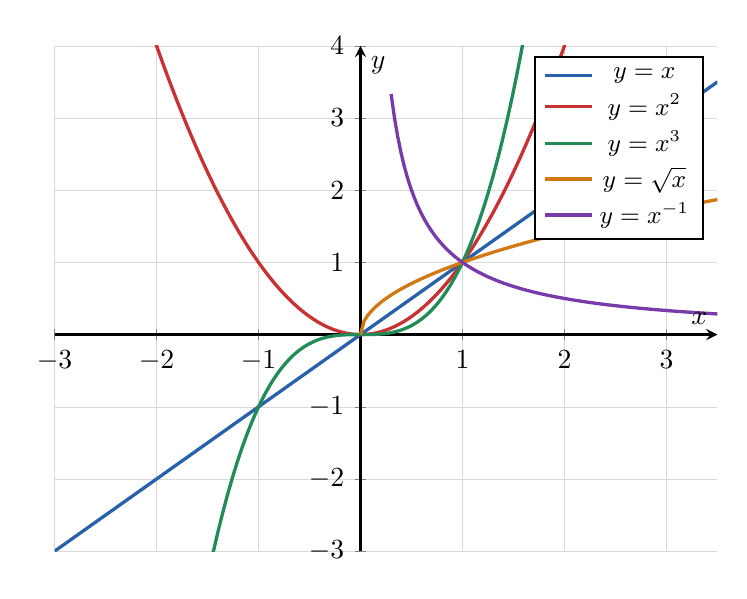
\begin{tikzpicture}
\begin{axis}[
    width=10cm, height=8cm,
    axis lines=middle,
    xlabel={$x$}, ylabel={$y$},
    xmin=-3, xmax=3.5,
    ymin=-3, ymax=4,
    samples=100,
    grid=both,
    grid style={line width=0.2pt, draw=gray!30},
    legend style={at={(0.98,0.98)}, anchor=north east, font=\small},
    thick,
]
\addplot[mainblue, very thick, domain=-3:3.5] {x};
\addlegendentry{$y=x$}
\addplot[warnred, very thick, domain=-2.2:2.2] {x^2};
\addlegendentry{$y=x^2$}
\addplot[tipgreen, very thick, domain=-2:2.6] {x^3};
\addlegendentry{$y=x^3$}
\addplot[examorange, very thick, domain=0:3.5] {sqrt(x)};
\addlegendentry{$y=\sqrt{x}$}
\addplot[apppurple, very thick, domain=0.3:3.5] {1/x};
\addlegendentry{$y=x^{-1}$}
\end{axis}
\end{tikzpicture}
\end{center}

\begin{tipbox}[幂函数与指数函数的区别]
\begin{itemize}[leftmargin=2em]
  \item \textbf{幂函数}：$y=x^\alpha$，底数是变量，指数是常数。
  \item \textbf{指数函数}：$y=a^x$，底数是常数，指数是变量。
  \item 两者形式不同，不要混淆！
\end{itemize}
\end{tipbox}


% =============================================================
%  第二部分：例题精讲
% =============================================================
\section*{\textcolor{examorange}{二、例题精讲}}

% ---- 例1 ----
\begin{examplebox}[【例1】根式与分数指数幂的互化]
将下列各式写成分数指数幂的形式：
\par (1) $\sqrt[5]{x^3}$ \qquad (2) $\dfrac{1}{\sqrt[3]{a}}$ \qquad (3) $\sqrt{a\sqrt{a}}$
\end{examplebox}

\textbf{解：}

(1) $\sqrt[5]{x^3} = x^{\frac{3}{5}}$

(2) $\dfrac{1}{\sqrt[3]{a}} = \dfrac{1}{a^{\frac{1}{3}}} = a^{-\frac{1}{3}}$

(3) 先把里面的根式化为分数指数幂：
\[
\sqrt{a\sqrt{a}} = \sqrt{a \cdot a^{\frac{1}{2}}} = \sqrt{a^{1+\frac{1}{2}}} = \sqrt{a^{\frac{3}{2}}} = a^{\frac{3}{2}\cdot\frac{1}{2}} = a^{\frac{3}{4}}
\]

\begin{tipbox}[方法总结]
根式化分数指数幂的步骤：(1) 先把各层根号化为 $\frac{1}{n}$ 次幂；(2) 利用幂的运算法则化简。
\end{tipbox}

% ---- 例2 ----
\begin{examplebox}[【例2】指数幂的化简计算]
计算下列各式：
\par (1) $\left(\dfrac{8}{27}\right)^{-\frac{2}{3}}$ \qquad (2) $0.064^{-\frac{1}{3}} - \left(-\dfrac{7}{8}\right)^{0} + 16^{0.75}$
\end{examplebox}

\textbf{解：}

(1)
\[
\left(\frac{8}{27}\right)^{-\frac{2}{3}} = \left(\frac{27}{8}\right)^{\frac{2}{3}} = \left(\left(\frac{3}{2}\right)^3\right)^{\frac{2}{3}} = \left(\frac{3}{2}\right)^{3 \times \frac{2}{3}} = \left(\frac{3}{2}\right)^{2} = \frac{9}{4}
\]

(2) 逐项计算：
\begin{itemize}[leftmargin=2em]
  \item $0.064^{-\frac{1}{3}} = \left(\dfrac{64}{1000}\right)^{-\frac{1}{3}} = \left(\dfrac{4}{10}\right)^{3 \times (-\frac{1}{3})} = \left(\dfrac{2}{5}\right)^{-1} = \dfrac{5}{2}$
  \item $\left(-\dfrac{7}{8}\right)^0 = 1$
  \item $16^{0.75} = 16^{\frac{3}{4}} = (2^4)^{\frac{3}{4}} = 2^3 = 8$
\end{itemize}

原式 $= \dfrac{5}{2} - 1 + 8 = \dfrac{3}{2} + 8 = \dfrac{19}{2}$

% ---- 例3 ----
\begin{examplebox}[【例3】判断指数函数的单调性]
比较下列各组数的大小：
\par (1) $1.7^{2.5}$ 与 $1.7^{3}$
\par (2) $0.8^{-0.1}$ 与 $0.8^{-0.2}$
\par (3) $2^{0.3}$ 与 $0.3^{2}$
\end{examplebox}

\textbf{解：}

(1) 底数 $1.7>1$，指数函数 $y=1.7^x$ 在 $\mathbb{R}$ 上单调递增。

因为 $2.5 < 3$，所以 $1.7^{2.5} < 1.7^{3}$。

(2) 底数 $0.8$，$0<0.8<1$，指数函数 $y=0.8^x$ 在 $\mathbb{R}$ 上单调递减。

因为 $-0.1 > -0.2$，所以 $0.8^{-0.1} < 0.8^{-0.2}$。

(3) 用中间值 $1$ 来"搭桥"：
\begin{itemize}[leftmargin=2em]
  \item $2^{0.3} > 2^0 = 1$ \quad（因为 $y=2^x$ 递增，$0.3>0$）
  \item $0.3^{2} = 0.09 < 1$
\end{itemize}
所以 $2^{0.3} > 0.3^{2}$。

\begin{tipbox}[方法总结]
比较指数幂大小的常用方法：\textbf{(1) 同底比较}——利用单调性；\textbf{(2) 中间值法}——用 $0$ 或 $1$ 做桥梁。
\end{tipbox}

% ---- 例4 ----
\begin{examplebox}[【例4】指数式与对数式的互化]
将下列指数式化为对数式，对数式化为指数式：
\par (1) $2^5 = 32$ \qquad (2) $\log_3 81 = 4$ \qquad (3) $\log_{\frac{1}{2}} 16 = -4$
\end{examplebox}

\textbf{解：}

(1) $2^5 = 32$ 化为对数式：$\log_2 32 = 5$

(2) $\log_3 81 = 4$ 化为指数式：$3^4 = 81$

(3) $\log_{\frac{1}{2}} 16 = -4$ 化为指数式：$\left(\dfrac{1}{2}\right)^{-4} = 16$

验证：$\left(\dfrac{1}{2}\right)^{-4} = 2^4 = 16$ \checkmark

% ---- 例5 ----
\begin{examplebox}[【例5】对数的运算]
计算下列各式：
\par (1) $\log_2 8 + \log_2 4$
\par (2) $\lg 100 + \ln \mathrm{e}^3$
\par (3) $\log_5 3 \times \log_9 25$
\end{examplebox}

\textbf{解：}

(1) 方法一（分别计算）：$\log_2 8 = 3$，$\log_2 4 = 2$，所以原式 $= 3+2=5$。

方法二（用法则）：$\log_2 8 + \log_2 4 = \log_2(8\times 4) = \log_2 32 = 5$。

(2) $\lg 100 = \lg 10^2 = 2$，$\ln \mathrm{e}^3 = 3$，所以原式 $= 2+3 = 5$。

(3) 利用换底公式：
\[
\log_5 3 \times \log_9 25 = \frac{\lg 3}{\lg 5} \times \frac{\lg 25}{\lg 9} = \frac{\lg 3}{\lg 5} \times \frac{2\lg 5}{2\lg 3} = 1
\]

\begin{tipbox}[方法总结]
对数计算三板斧：(1) 能直接算的先算（如 $\log_2 8=3$）；(2) 用运算法则合并；(3) 底数不同时用换底公式统一。
\end{tipbox}

% ---- 例6 ----
\begin{examplebox}[【例6】对数函数的定义域与值域]
求下列函数的定义域：
\par (1) $y = \log_2(x-1)$ \qquad (2) $y = \log_3(9-x^2)$ \qquad (3) $y = \dfrac{1}{\sqrt{\log_{\frac{1}{2}} x}}$
\end{examplebox}

\textbf{解：}

(1) 对数的真数必须大于 $0$：
\[
x - 1 > 0 \implies x > 1
\]
定义域为 $(1, +\infty)$。

(2) 真数大于 $0$：
\[
9 - x^2 > 0 \implies x^2 < 9 \implies -3 < x < 3
\]
定义域为 $(-3, 3)$。

(3) 需要满足两个条件：
\begin{itemize}[leftmargin=2em]
  \item 真数 $x>0$
  \item 分母 $\sqrt{\log_{\frac{1}{2}} x}$ 有意义且不为零，即 $\log_{\frac{1}{2}} x > 0$
\end{itemize}

由 $\log_{\frac{1}{2}} x > 0$，因为 $0<\frac{1}{2}<1$，函数递减，所以 $0 < x < 1$。

结合 $x>0$，定义域为 $(0, 1)$。

% ---- 例7 ----
\begin{examplebox}[【例7】比较对数的大小]
比较下列各组数的大小：
\par (1) $\log_2 3$ 与 $\log_2 5$
\par (2) $\log_3 2$ 与 $\log_5 2$
\par (3) $\log_2 0.3$，$2^{0.3}$，$0.3^{2}$ 三者从小到大排列
\end{examplebox}

\textbf{解：}

(1) 底数 $2>1$，$y=\log_2 x$ 在 $(0,+\infty)$ 上递增。

因为 $3<5$，所以 $\log_2 3 < \log_2 5$。

(2) 底数不同，借助中间值 $1$：因为 $2>1$，所以 $\log_3 2 > \log_3 1 = 0$ 且 $\log_5 2 > \log_5 1 = 0$。

用换底公式更直接：
\[
\log_3 2 = \frac{1}{\log_2 3}, \quad \log_5 2 = \frac{1}{\log_2 5}
\]
因为 $\log_2 3 < \log_2 5$，取倒数后 $\dfrac{1}{\log_2 3} > \dfrac{1}{\log_2 5}$。

所以 $\log_2 3 > \log_5 2$。

(3) 逐个判断：
\begin{itemize}[leftmargin=2em]
  \item $\log_2 0.3$：$0<0.3<1$，底数 $2>1$，所以 $\log_2 0.3 < 0$
  \item $0.3^2 = 0.09$，满足 $0 < 0.09 < 1$
  \item $2^{0.3} > 2^0 = 1$
\end{itemize}

从小到大：$\log_2 0.3 < 0.3^2 < 2^{0.3}$

\begin{tipbox}[方法总结]
"三大"比较策略：(1) 同底同类型利用单调性；(2) 不同类型借助中间值 $0$ 或 $1$；(3) 换底公式统一底数。
\end{tipbox}

% ---- 例8 ----
\begin{examplebox}[【例8】指数函数与对数函数的综合]
已知函数 $f(x) = a^x$（$a>0$，$a\neq 1$）的图象过点 $(2, 9)$。

(1) 求 $f(x)$ 的解析式；

(2) 求 $f(-1)$，$f(0)$，$f\!\left(\frac{1}{2}\right)$ 的值；

(3) 若 $f(x) \geq 27$，求 $x$ 的取值范围。
\end{examplebox}

\textbf{解：}

(1) 将 $(2,9)$ 代入 $f(x)=a^x$：
\[
a^2 = 9 \implies a = 3 \quad (\text{因为 } a>0)
\]
所以 $f(x) = 3^x$。

(2)
\begin{itemize}[leftmargin=2em]
  \item $f(-1) = 3^{-1} = \dfrac{1}{3}$
  \item $f(0) = 3^0 = 1$
  \item $f\!\left(\dfrac{1}{2}\right) = 3^{\frac{1}{2}} = \sqrt{3}$
\end{itemize}

(3) $3^x \geq 27 = 3^3$

因为 $y=3^x$ 是增函数，所以 $x \geq 3$。

$x$ 的取值范围为 $[3, +\infty)$。

\begin{tipbox}[方法总结]
指数函数过已知点可求底数；解指数不等式的关键是化为\textbf{同底}，再利用单调性去掉底数。
\end{tipbox}

% ---- 例9 ----
\begin{examplebox}[【例9】对数方程]
解下列方程：
\par (1) $\log_3(2x+1) = 2$
\par (2) $\lg(x+3) + \lg(x-3) = \lg 7$
\end{examplebox}

\textbf{解：}

(1) 化为指数式：
\[
2x + 1 = 3^2 = 9 \implies 2x = 8 \implies x = 4
\]

验证：真数 $2(4)+1 = 9 > 0$ \checkmark，所以 $x=4$。

(2) 利用对数运算法则：
\[
\lg[(x+3)(x-3)] = \lg 7
\]
\[
(x+3)(x-3) = 7
\]
\[
x^2 - 9 = 7 \implies x^2 = 16 \implies x = \pm 4
\]

验证真数条件：
\begin{itemize}[leftmargin=2em]
  \item $x=4$：$x+3=7>0$，$x-3=1>0$ \checkmark
  \item $x=-4$：$x-3=-7<0$，不满足 \texttimes
\end{itemize}

所以 $x=4$。

\begin{warnbox}[解对数方程的关键]
解对数方程后，\textbf{必须验证}真数是否大于零！这是最容易丢分的步骤。
\end{warnbox}


% =============================================================
%  第三部分：应用题
% =============================================================
\section*{\textcolor{apppurple}{三、应用题}}

% ---- 应用1 ----
\begin{appbox}[【应用1】细菌繁殖模型]
某种细菌每过 $20$ 分钟便由 $1$ 个分裂成 $2$ 个（即数量翻倍）。现有 $1$ 个这种细菌。

(1) 写出经过 $t$ 分钟后细菌个数 $y$ 关于 $t$ 的函数关系式；

(2) 经过多少时间后，细菌数量可达 $1024$ 个？
\end{appbox}

\textbf{解：}

(1) 每 $20$ 分钟翻倍一次，经过 $t$ 分钟翻倍了 $\dfrac{t}{20}$ 次。

所以 $y = 1 \times 2^{\frac{t}{20}} = 2^{\frac{t}{20}}$（$t\geq 0$）。

(2) 当 $y=1024$ 时：
\[
2^{\frac{t}{20}} = 1024 = 2^{10}
\]
\[
\frac{t}{20} = 10 \implies t = 200 \text{（分钟）}
\]

答：经过 $200$ 分钟（即 $3$ 小时 $20$ 分钟）后，细菌数量可达 $1024$ 个。

% ---- 应用2 ----
\begin{appbox}[【应用2】地震震级与对数]
地震的里氏震级 $M$ 的计算公式为 $M = \lg A - \lg A_0$，其中 $A$ 是地震仪记录到的最大振幅，$A_0$ 是标准振幅。

(1) 若某次地震的振幅是标准振幅的 $1000$ 倍，求这次地震的震级；

(2) 2008 年汶川地震约为 $8.0$ 级，2010 年玉树地震约为 $7.1$ 级。$8.0$ 级地震的振幅大约是 $7.1$ 级地震振幅的多少倍？
\end{appbox}

\textbf{解：}

(1) $M = \lg \dfrac{A}{A_0} = \lg 1000 = \lg 10^3 = 3$

答：这次地震的震级为 $3$ 级。

(2) 设 $8.0$ 级地震振幅为 $A_1$，$7.1$ 级地震振幅为 $A_2$。

\[
M_1 = \lg \frac{A_1}{A_0} = 8.0, \quad M_2 = \lg \frac{A_2}{A_0} = 7.1
\]
\[
\lg \frac{A_1}{A_0} - \lg \frac{A_2}{A_0} = 8.0 - 7.1 = 0.9
\]
\[
\lg \frac{A_1}{A_2} = 0.9 \implies \frac{A_1}{A_2} = 10^{0.9} \approx 7.94
\]

答：$8.0$ 级地震的振幅大约是 $7.1$ 级地震振幅的 $8$ 倍（约 $7.94$ 倍）。

\begin{tipbox}[生活中的对数]
震级每增加 $1$ 级，振幅增大约 $10$ 倍；$M_1 - M_2 = 0.9$，振幅比为 $10^{0.9}\approx 8$ 倍。对数将巨大的倍数关系压缩为小数字，这就是震级用对数定义的原因。
\end{tipbox}

% ---- 应用3 ----
\begin{appbox}[【应用3】溶液稀释问题]
一杯含盐 $20\%$ 的盐水共 $200$ 克。现在不断往里加清水（每次加 $200$ 克），每次加完充分搅拌后倒出 $200$ 克混合液。

设第 $n$ 次操作后盐水的浓度为 $p_n$。

(1) 求 $p_n$ 与 $n$ 的函数关系；

(2) 至少操作几次后，浓度低于 $5\%$？

\textbf{（提示：每次操作后剩余盐量变为原来的 $\dfrac{1}{2}$）}
\end{appbox}

\textbf{解：}

(1) 每次操作，盐水总量保持 $200$ 克，但盐量变为原来的 $\dfrac{200}{400} = \dfrac{1}{2}$（加入 $200$ 克水后总量 $400$ 克，倒出 $200$ 克即倒出一半）。

初始盐量 $= 200 \times 20\% = 40$ 克。

第 $n$ 次操作后盐量 $= 40 \times \left(\dfrac{1}{2}\right)^n$ 克。

浓度：$p_n = \dfrac{40 \times (\frac{1}{2})^n}{200} = 20\% \times \left(\dfrac{1}{2}\right)^n = 0.2 \times \left(\dfrac{1}{2}\right)^n$

(2) 令 $p_n < 5\% = 0.05$：
\[
0.2 \times \left(\frac{1}{2}\right)^n < 0.05
\]
\[
\left(\frac{1}{2}\right)^n < \frac{0.05}{0.2} = \frac{1}{4} = \left(\frac{1}{2}\right)^2
\]

因为底数 $0<\frac{1}{2}<1$，指数函数递减，所以 $n>2$。

答：至少操作 $3$ 次后，浓度低于 $5\%$。


% =============================================================
%  第四部分：课堂练习
% =============================================================
\section*{\textcolor{tipgreen}{四、课堂练习}}

\begin{enumerate}[leftmargin=2em, label=\textbf{\arabic*.}]
  \item 计算：$8^{\frac{2}{3}} + \left(\dfrac{1}{2}\right)^{-2} - (\pi - 3)^{0}$

  \item 化简：$\dfrac{a^{\frac{1}{2}} \cdot a^{\frac{3}{2}}}{a^2}$（$a>0$）

  \item 已知 $2^x = \dfrac{1}{8}$，求 $x$ 的值。

  \item 求值：$\log_3 27 - \log_3 9 + \log_3 1$

  \item 已知 $\lg 2 \approx 0.3010$，$\lg 3 \approx 0.4771$，求 $\lg 12$ 的近似值。

  \item 求函数 $y = \log_5(2x-6)$ 的定义域。

  \item 比较大小：$\log_2 0.5$ \underline{\qquad} $0$，$\log_{0.3} 2$ \underline{\qquad} $0$（填 "$>$"、"$<$" 或 "$=$"）。

  \item 已知函数 $f(x)=a^x$（$a>0$，$a\neq 1$）在 $[-1,1]$ 上的最大值与最小值之差为 $\dfrac{8}{3}$，求 $a$ 的值。
\end{enumerate}

\vspace{20pt}
\begin{knowledgebox}[参考答案]
\begin{enumerate}[leftmargin=2em, label=\textbf{\arabic*.}]

  \item $8^{\frac{2}{3}} = (2^3)^{\frac{2}{3}} = 2^2 = 4$，$\left(\dfrac{1}{2}\right)^{-2} = 2^2 = 4$，$(\pi-3)^0 = 1$。\par
  原式 $= 4 + 4 - 1 = \mathbf{7}$。

  \item $\dfrac{a^{\frac{1}{2}} \cdot a^{\frac{3}{2}}}{a^2} = \dfrac{a^{\frac{1}{2}+\frac{3}{2}}}{a^2} = \dfrac{a^2}{a^2} = \mathbf{1}$。

  \item $2^x = \dfrac{1}{8} = 2^{-3}$，所以 $x = \mathbf{-3}$。

  \item $\log_3 27 = 3$，$\log_3 9 = 2$，$\log_3 1 = 0$。\par
  原式 $= 3 - 2 + 0 = \mathbf{1}$。

  \item $\lg 12 = \lg(4\times 3) = \lg 4 + \lg 3 = 2\lg 2 + \lg 3 = 2\times 0.3010 + 0.4771 = \mathbf{1.0791}$。

  \item 需 $2x-6>0$，即 $x>3$。定义域为 $\mathbf{(3, +\infty)}$。

  \item $\log_2 0.5 = \log_2 2^{-1} = -1 < 0$，填 $\mathbf{<}$。\par
  $\log_{0.3} 2$：底数 $0<0.3<1$，$2>1$，所以 $\log_{0.3} 2 < 0$，填 $\mathbf{<}$。

  \item \textbf{情形一}：$a>1$ 时，$f(x)=a^x$ 在 $[-1,1]$ 上递增。\par
  最大值 $a^1 = a$，最小值 $a^{-1} = \dfrac{1}{a}$。\par
  $a - \dfrac{1}{a} = \dfrac{8}{3}$，即 $3a^2 - 8a - 3 = 0$，$(3a+1)(a-3)=0$。\par
  $a=3$ 或 $a=-\dfrac{1}{3}$（舍去），故 $a=\mathbf{3}$。\par
  \textbf{情形二}：$0<a<1$ 时，$f(x)=a^x$ 在 $[-1,1]$ 上递减。\par
  最大值 $a^{-1}=\dfrac{1}{a}$，最小值 $a^1=a$。\par
  $\dfrac{1}{a}-a=\dfrac{8}{3}$，即 $3a^2+8a-3=0$，$(3a-1)(a+3)=0$。\par
  $a=\dfrac{1}{3}$ 或 $a=-3$（舍去），故 $a=\mathbf{\dfrac{1}{3}}$。\par
  综上，$a = 3$ 或 $a = \dfrac{1}{3}$。

\end{enumerate}
\end{knowledgebox}

\vfill
\begin{center}
\small\textcolor{gray}{本讲义仅供教学参考，例题可根据学生水平调整难度。}
\end{center}

\end{document}
